
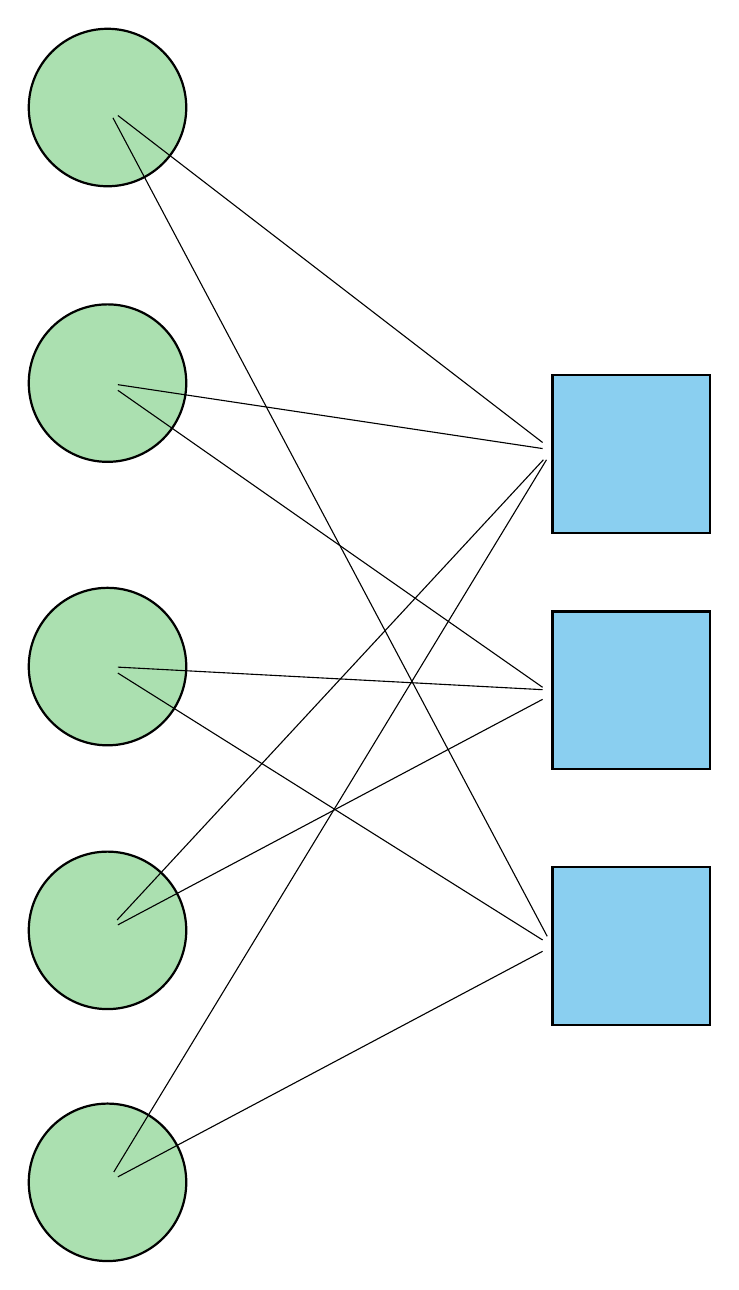
\begin{tikzpicture}

\definecolor{brightturquoise}{rgb}{0.03, 0.91, 0.87}
\definecolor{buff}{rgb}{0.94, 0.86, 0.51}
\definecolor{caribbeangreen}{rgb}{0.0, 0.8, 0.6}
\definecolor{celadon}{rgb}{0.67, 0.88, 0.69}
\definecolor{darktangerine}{rgb}{1.0, 0.66, 0.07}
\definecolor{darkviolet}{rgb}{0.58, 0.0, 0.83}
\definecolor{deepskyblue}{rgb}{0.0, 0.75, 1.0}
\definecolor{amber(sae/ece)}{rgb}{1.0, 0.49, 0.0}
\definecolor{antiquewhite}{rgb}{0.98, 0.92, 0.84}
\definecolor{applegreen}{rgb}{0.55, 0.71, 0.0}
\definecolor{babyblue}{rgb}{0.54, 0.81, 0.94}

% Variable nodes 
\draw [thick,fill=celadon]   (-7,-5.55) node (v6) {} ellipse (1 and 1);
\draw[thick,fill=celadon]  (-7,-2.2) node (v5) {} ellipse (1 and 1);
\draw [thick,fill=celadon]  (-7,1.4) node (v3) {} ellipse (1 and 1);
\draw  [thick,fill=celadon]  (-7,-8.75) node (v1) {} ellipse (1 and 1);
\draw  [thick,fill=celadon]  (-7,4.9) node (v1_2) {} ellipse (1 and 1);
%Check nodes



\draw [thick,fill=babyblue]  (-1.35,1.5) node (v8) {} rectangle (0.65,-0.5);
\draw [thick,fill=babyblue] (-1.35,-1.5) rectangle (0.65,-3.5);
\draw [thick,fill=babyblue] (-1.35,-4.75) rectangle (0.65,-6.75);










\node (v2) at (-1.35,0.55) {};
\node (v4) at (-1.35,-2.5) {};


\node (v7) at (-1.35,-5.75) {};
\node (v9) at (-1.35,-2.55) {};

\draw  (v1_2) edge (v2);
\draw  (v1_2) edge (v7);

\draw  (v3) edge (v9);
\draw  (v5) edge (v4);
\node (v12) at (-1.35,0.55) {};
\draw  (v3) edge (v12);
\draw  (v5) edge (v7);

\draw  (v6) edge (v2);
\draw  (v1) edge (v12);
\draw  (v6) edge (v9);
\draw  (v1) edge (v7);
\end{tikzpicture}
